For $q_1$, the truth table
\begin{table}[h]
    \centering
    \begin{tabular}{|c|c|c|c|}
    \hline
         $A$ & $B$ & $C$ & $(AB) + C$ \\
         \hline
         1 &1  & 0 &1\\\hline
         1&1&1&1\\\hline
         0&1&1&1\\\hline
         0&0&1&1\\\hline
         1&0&1&1\\
    \hline
    \end{tabular}
    \caption{Circuit 1 working}
    \label{june2016-118:tab:my_label}
\end{table}
Multiplying and adding probability for each case of $q_1$ gives us the value of $q_1$ as
\begin{align}
    q_1 = p^3-2p^2+1
\end{align}
For $q_2$, the truth table
\begin{table}[h]
    \centering
    \begin{tabular}{|c|c|c|c|}
    \hline
         $A$ & $B$ & $C$ & $(A+B)C$ \\
         \hline
         1&1&1&1\\ \hline
         1&0&1&1\\\hline
         0&1&1&1\\
    \hline
    \end{tabular}
    \caption{Circuit 2 working}
    \label{june2016-118:tab:table2}
\end{table}
Multiplying and adding probability for each case of $q_2$ gives us the value of $q_2$ as
\begin{align}
    q_2 = p^3-p^2-p+1
\end{align}
For $q_3$, the truth table
\begin{table}[h]
    \centering
    \begin{tabular}{|c|c|c|c|}
    \hline
         $A$ & $B$ & $C$ & $A + B + C$ \\
         \hline
         1&0&0&1\\\hline
         0&1&0&1\\\hline
         0&0&1&1\\\hline
         1&1&0&1\\\hline
         1&0&1&1\\\hline
         0&1&1&1\\\hline
         1&1&1&1\\
    \hline
    \end{tabular}
    \caption{Circuit 3 working}
    \label{june2016-118:tab:table3}
\end{table}
Multiplying and adding probability for each case of $q_3$ gives us the value of $q_3$ as
\begin{align}
    q_3 = 1-p^3
\end{align}
%%
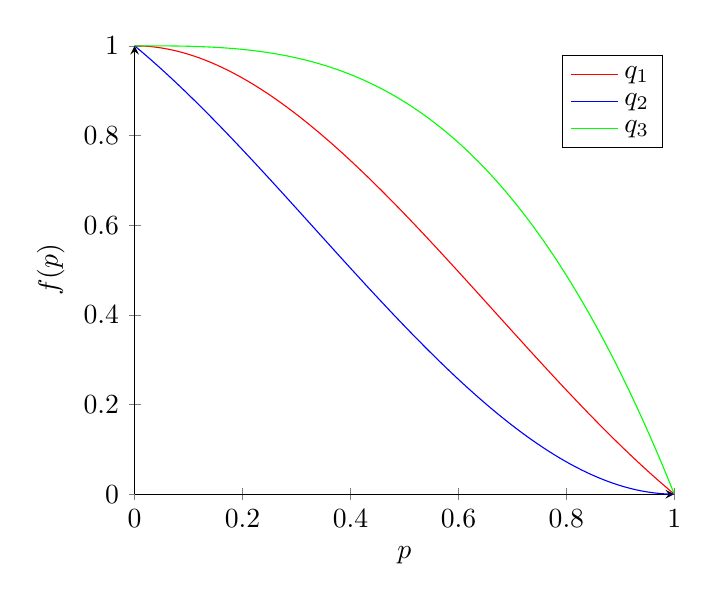
\begin{tikzpicture}
\begin{axis}[
    axis lines = left,
    xlabel = $p$,
    ylabel = {$f(p)$},
]
\addplot [
    domain=0:1, 
    samples=100, 
    color=red,
]
{x^3-2*x^2+1};
\addlegendentry{$q_1$}
\addplot [
    domain=0:1, 
    samples=100, 
    color=blue,
    ]
    {x^3-x^2-x+1};
\addlegendentry{$q_2$}
\addplot [
    domain=0:1, 
    samples=100, 
    color=green,
]
{1-x^3};
\addlegendentry{$q_3$}
\end{axis}
\end{tikzpicture}
\begin{align}
    \therefore q_3>q_1>q_2
\end{align}
Hence \textbf{Option 1} is correct